% IEEE conference paper (IEEEtran), at most 6 pages. Compile: pdflatex main; bibtex main; pdflatex main; pdflatex main
% (or tectonic -X compile main.tex). Every number is copied from a saved analysis table in results/phase2/.
\documentclass[conference]{IEEEtran}
\usepackage[T1]{fontenc}
\usepackage{newtxtext,newtxmath}  % Times text and math (works with pdflatex and XeTeX)
\usepackage{amsmath}
\usepackage{graphicx}
\usepackage{booktabs}
\usepackage{cite}
\usepackage[hidelinks]{hyperref}
\graphicspath{{figures/}}

\begin{document}
\bstctlcite{IEEEexample:BSTcontrol}

\title{Uncertainty-Aware Runtime Assurance for Safe Learning-Based Planetary Rover Navigation Under Distribution Shift}

\author{
\IEEEauthorblockN{Zoyba Parihan}
\IEEEauthorblockA{Dept. of CSE(AI\&ML)\\
Dayananda Sagar University\\
Bangalore, India\\
zoybaparihan006@gmail.com}
\and
\IEEEauthorblockN{Abubakar Zibran Shabir Sheikh}
\IEEEauthorblockA{Dept. of CSE(AI\&ML)\\
Dayananda Sagar University\\
Bangalore, India\\
zibran.shaikh99@gmail.com}
\and
\IEEEauthorblockN{Archita Bhattacharyya}
\IEEEauthorblockA{Dept. of Cybersecurity\\
Dayananda Sagar University\\
Bangalore, India\\
architabhattacharyya-cs@dsu.edu.in}
}

\maketitle

\begin{abstract}
Learned navigation policies can drive a rover efficiently but may fail silently when terrain, sensing or dynamics differ
from training. We study an onboard runtime-assurance layer in which a five-member deep-Q ensemble proposes each move,
executed only if an ensemble-disagreement check, an out-of-distribution (OOD) check and explicit safety rules all pass;
otherwise a battery-aware A* planner takes over or the rover stops safely. In a $32\times32$ partially observable
simulator with four kinds of shift, under a frozen, pre-registered protocol, the assured system attempts the fewest unsafe
moves of all baselines in every condition (77--99\% fewer than the unshielded ensemble) but does not reach the success of
plain A*. The safety rules provide most of the gain; a
raw-observation OOD check fires on 94\% of decisions under sensor shift and degrades results, an action-conditioned OOD
score removes this harm without adding value, and an energy-aware fallback is decisive under combined shift. On 450 maps
from HiRISE terrain models of three rover sites, the assured system matches A* in success with 81\% fewer unsafe moves
under nominal physics, but not under shifted physics. All results are from simulation.
\end{abstract}

\begin{IEEEkeywords}
runtime assurance, safe reinforcement learning, out-of-distribution detection, deep ensembles, planetary rover
\end{IEEEkeywords}

% =====================================================================================================================
\section{Introduction}
Autonomy has become central to planetary exploration. Perseverance evaluated most of its first Mars year of driving
with its onboard navigation system~\cite{verma2023perseverance}, and learning-based planners and traversability models
are now studied as a way to drive farther and more efficiently~\cite{daftry2022mlnav,endo2023risk,miao2025review}.
Yet any learned component will eventually face conditions it was not trained on, and this paper studies how to keep
it in use while preventing harm when it should not be trusted.

\subsection{Motivation}
Commands from Earth arrive minutes late and are uplinked only a few times per day, so a rover that waits for the ground
before every move covers little distance. Learned policies can make efficient local decisions in cluttered terrain and
trade distance against energy without hand-tuned costs~\cite{tanaka2024lunar}, but their value estimates are reliable
only near the states they were trained on~\cite{kirk2023generalisation}. A rover may meet terrain rougher than any
training map, a camera degraded by dust or lighting, or soil that is costlier to cross than expected, and a learned
policy can then choose a move that looks good to it but is unsafe or leaves too little energy to finish the traverse.
Because the rover sees only a small window around itself and must keep a battery reserve, such errors are hard to detect
onboard and expensive when they occur. Runtime assurance (RTA) keeps the learned controller in charge only while a
supervisor trusts it and hands control to a simpler fallback otherwise~\cite{hobbs2023rta,wabersich2023safety}, but it is
unclear which signals should trigger an intervention on a rover, what the fallback should optimise, and how much mission
performance is traded for safety.

\subsection{Contributions}
The contributions of this paper are:
\begin{enumerate}
\item an RTA architecture for a learned rover navigator whose components use only onboard information;
\item a frozen, pre-registered evaluation of 18 methods and variants over five shift conditions, which identifies the
safety rules as the main source of safety and shows that a raw OOD check is harmful under sensor shift;
\item follow-up experiments showing that an action-conditioned OOD score repairs this failure but adds no value, and that
an energy-aware fallback is decisive under combined shift;
\item a transfer test on 450 maps derived from Mars elevation data at three rover sites.
\end{enumerate}

% =====================================================================================================================
\section{Related Work}
\subsection{Runtime Assurance and Safe Learning}
RTA filters the output of an unverified controller and switches to a trusted backup when safety is at
risk~\cite{hobbs2023rta}. Neural Simplex~\cite{phan2020neuralsimplex} and Black-Box Simplex~\cite{mehmood2022bbsimplex}
apply this idea to learned controllers, and data-driven safety filters based on reachability, control barrier functions
or predictive control generalise it to uncertain systems~\cite{wabersich2023safety}. In reinforcement learning, shields
restrict an agent to actions certified as safe, also under partial observability~\cite{carr2023pomdpshield}, and recent
reviews survey safe RL and safe robot learning more broadly~\cite{gu2024saferl,brunke2022saferobot}. These approaches
mostly switch on explicit safety conditions; we combine such rules with learned-confidence checks and an energy budget,
without a formal guarantee.

\subsection{Uncertainty and Out-of-Distribution Detection}
Ensembles are a standard way to quantify epistemic uncertainty in deep learning~\cite{abdar2021uq} and have been used to
weight and guide value learning in deep RL~\cite{lee2021sunrise}. OOD detection is surveyed in~\cite{yang2024ood}, which
covers the feature-space Mahalanobis detectors used here, and has been adapted to RL agents through probabilistic dynamics
ensembles~\cite{haider2023ood}. Deep RL generalises poorly to unseen environment variations~\cite{kirk2023generalisation}; we treat all
scores as uncalibrated.

\subsection{Planetary Rover Navigation}
Perseverance's onboard autonomy~\cite{verma2023perseverance} shows the operational value of self-driving rovers. Learning
has been applied to Martian terrain classification~\cite{swan2021ai4mars}, to learned path planning with a safety check on
Martian terrain~\cite{daftry2022mlnav}, to risk-aware planning from probabilistic traversability~\cite{endo2023risk}, and
to resource-constrained global planning with deep RL~\cite{tanaka2024lunar}; Miao and Wei~\cite{miao2025review} review
rover path planning. We found no study that wraps a learned rover navigator in an RTA layer and measures intervention,
safe-stop and energy trade-offs under controlled shifts by ablation.

% =====================================================================================================================
\section{Methodology}
Fig.~\ref{fig:arch} summarises the assurance layer described in this section.

\begin{figure}[t]
\centering
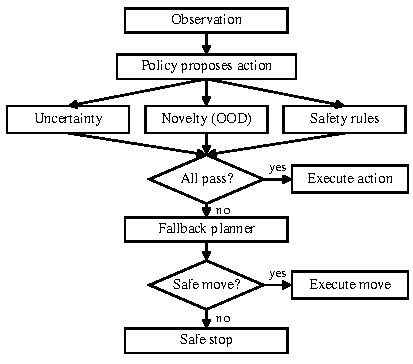
\includegraphics[width=\columnwidth]{fig1_architecture}
\caption{Architecture of the runtime-assurance layer. At every step the ensemble's proposed action is executed only if all
three checks pass; otherwise the battery-aware fallback acts, or the rover stops safely.}
\label{fig:arch}
\end{figure}

\subsection{Environment and Observations}
The world is a $32\times32$ grid of normal, sand and rock cells and impassable obstacles, generated from smoothed noise
fields (Table~\ref{tab:sim}). The rover starts at $(0,0)$ with battery $B_0=250$ and must reach $(31,31)$ using four
compass moves. Entering a cell costs 1, 3 or 5 illustrative energy units for normal, sand or rock; a terrain-dependent
slip replaces the commanded move by a perpendicular one, and a collision costs one unit without moving the rover.

The rover observes a 59-dimensional vector: position and goal offset, battery and step fractions, an odometry-based slip
estimate, a sensor self-consistency score, map coverage, a noisy $5\times5$ terrain reading and its own visit counts.
Readings miss obstacles, report false ones and carry Gaussian noise, and the rover keeps an explored map of its readings
and collisions. All onboard components use only the observation and this map; ground truth is visible only to the
evaluator, which automated tests enforce (Fig.~\ref{fig:episode}). An episode ends at the goal, at battery depletion, or
at a safe stop, which counts as a failure. We count collisions and attempted unsafe moves (commanded moves into an
obstacle or off the map). Policies are trained in-distribution (ID); four test-time shifts change the hidden parameters
(Table~\ref{tab:sim}): terrain, sensor, dynamics and all three combined.

\begin{figure*}[t]
\centering
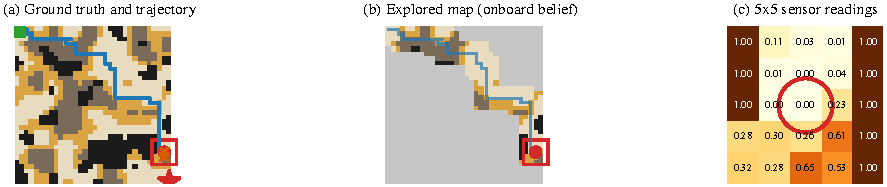
\includegraphics[width=\textwidth]{fig2_episode}
\caption{Example episode of the assured system on a debugging map under terrain shift, shown at its first intervention.
Fallback steps are marked x; grey cells in (b) are unknown to the rover.}
\label{fig:episode}
\end{figure*}

\begin{table}[t]
\centering
\caption{Simulator parameters per condition (n/s/r: normal/sand/rock).}
\label{tab:sim}
\setlength{\tabcolsep}{2pt}
\footnotesize
\begin{tabular}{@{}lccccc@{}}
\toprule
Parameter & ID & Terrain & Sensor & Dyn. & Comb. \\ \midrule
Mix (n/s/r) & .60/.15/.10 & .35/.25/.22 & .60/.15/.10 & .60/.15/.10 & .35/.25/.22 \\
Obstacles & .15 & .18 & .15 & .15 & .18 \\
Energy (n/s/r) & 1/3/5 & 1/3/5 & 1/3/5 & 1/4/6 & 1/4/6 \\
Slip (n/s/r) & .02/.10/.05 & .02/.10/.05 & .02/.10/.05 & .06/.25/.15 & .06/.25/.15 \\
Miss/false & .05/.02 & .05/.02 & .20/.08 & .05/.02 & .20/.08 \\
Noise $\sigma$ & .05 & .05 & .15 & .05 & .15 \\ \bottomrule
\end{tabular}
\end{table}

\subsection{Runtime-Assurance Controller}
The policy is an ensemble of $K=5$ Double-DQN members, each with a fixed randomised prior network and bootstrap weights
on replayed transitions, so that the members disagree away from the training data~\cite{abdar2021uq,lee2021sunrise}. The
proposed action $a_t$ maximises the member-mean Q-value, and its uncertainty is $u_t=\mathrm{std}_k\,Q_k(o_t,a_t)$. The
OOD check is a Mahalanobis detector~\cite{yang2024ood} on the observation features whose score $s_t$ is averaged over the
last 10 steps. The thresholds $\tau_u$ and $\tau_s$ are the 95th percentiles of $u_t$ and $s_t$ on ID validation maps.

The safety rules veto a move that leaves the map; targets a cell read as an obstacle, believed blocked by most past
readings, or proven blocked by a collision; costs more nominal energy than the battery holds or leaves less battery than
the Manhattan distance to the goal; or risks a sideways slip into a blocked cell when the slip estimate is at least 0.15.
The first three rules also screen the fallback's moves. The fallback is a battery-aware A* planner on the explored map:
known cells cost their nominal energy, unknown cells cost 2 plus a risk premium that grows as the battery drains, and
cells proven blocked are walls. It takes the best-ranked move that passes the rules; if the cheapest estimated route
needs more energy than remains, or every move is vetoed, the rover performs a safe stop.

\subsection{Action-Conditioned OOD Score}
To test a diagnosis of the OOD failure (Section~\ref{sec:a3}), a variant replaces only the OOD score with a
class-conditional Mahalanobis distance~\cite{yang2024ood} on each member's last hidden layer, using the proposed action as
the class and averaging over members. Fitting data, shrinkage, window and threshold rule are unchanged.

\subsection{Real-Terrain Maps}
To test transfer, we built maps from three public HiRISE digital terrain models at rover sites: Victoria crater
(Opportunity), Jezero crater (Perseverance) and Gale crater (Curiosity). Elevations were averaged to 2\,m cells. A cell is
an obstacle if its slope exceeds $25^\circ$ or its local relief exceeds the site's 97th percentile, rock if its slope is
15--25$^\circ$, sand if its slope is below $5^\circ$ and its relief below the 20th percentile, and normal otherwise. We kept
fully valid, non-overlapping $32\times32$ tiles that pass the simulator's acceptance rule (at most 300 per site), half for
debugging and 450 for evaluation. The rule encodes terrain structure, not traversability; real terrain is flatter, with
3--7\% obstacle cells against 15\% in the procedural maps (Fig.~\ref{fig:tiles}).

\begin{figure}[t]
\centering
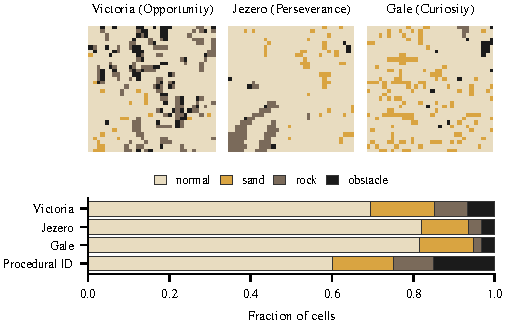
\includegraphics[width=\columnwidth]{fig10_real_tiles}
\caption{Real-terrain maps from HiRISE terrain models at the Opportunity, Perseverance and Curiosity sites (2\,m cells):
one evaluation tile per site and the terrain composition compared with the procedural ID generator.}
\label{fig:tiles}
\end{figure}

% =====================================================================================================================
\section{Implementation}
\subsection{Software and Training}
The simulator, planners and assurance layer are written in Python with NumPy, and the networks in PyTorch. Each ensemble
member has hidden layers $(256,256,128)$, discount 0.99, learning rate $5\times10^{-4}$, batch size 128, a 50{,}000-transition
replay buffer, 2{,}000 warm-up steps, target updates every 500 steps, gradient clipping at 1.0 and $\epsilon$-greedy
exploration decaying from 1.0 to 0.05 by 0.992 per episode. The randomised prior is a fixed $(64,64)$ network scaled by 10,
and transitions receive Poisson(1) bootstrap weights. Members train independently for 1{,}500 ID episodes, keeping the
checkpoint with the best success on 50 validation maps. PPO uses two 256-unit layers, clipping 0.2, GAE ($\lambda=0.95$), 512-step rollouts and the same budget.

The Mahalanobis detector (shrinkage 0.1) is fitted on plain-ensemble observations from 200 fitting maps, and both
thresholds are set on 100 ID validation maps separately for each of the 10 ensembles.

\subsection{Baselines and Variants}
The baselines are battery-aware A* on the explored map; A*+monitor, which has the assured system's rules, fallback and
safe stop but no learned component; a reactive explorer using only the sensor window; DQN and PPO, each with and without a
rule shield that replaces unsafe actions by the best safe one; the plain ensemble; and an uncertainty-gated ensemble. The
assured system is run with and without safe stop, and eight variants remove or isolate the checks and rules or change the
threshold percentile.

\subsection{Protocol and Statistics}
Maps are split into disjoint training, validation, fitting, testing and confirmatory sets. All results use the
confirmatory set (500 maps per condition), untouched until code, models, thresholds and analysis plan were frozen and
hashed; every method sees the same maps in the same order. The energy-blind fallback,
action-conditioned OOD and real-terrain experiments were added later as pre-registered amendments, each frozen before its
own data existed, and before each one a frozen result was reproduced byte for byte. We report means with 95\%
$t$-intervals over 10 seeds (Wilson intervals over maps for A*) and compare methods paired by seed on identical maps, using
exact sign-flip permutation tests with Holm--Bonferroni correction across conditions. All runs used one thread per job on
a laptop CPU (Apple M5), 28.2 core-hours in total.

% =====================================================================================================================
\section{Results}
\subsection{Main Comparison}
Fig.~\ref{fig:main} and Table~\ref{tab:main} report success and attempted unsafe moves. The assured system attempts the
fewest unsafe moves of all baselines in every condition, for example 0.035 per episode ID against 1.99 for the plain
ensemble and 0.096 for A*+monitor, and has fewer collisions than every baseline. Plain A*, however, succeeds significantly more often in all
conditions (by 1.6 to 8.8 points) while attempting 8--14 times more unsafe moves in the ID, terrain and dynamics
conditions; against A*+monitor, success differs significantly only under terrain shift ($-2.3$ points). The learned
proposer's benefit over the same planner is thus lower unsafe exposure and energy use (94.7 against 101.2 units ID;
Fig.~\ref{fig:ops}a), not higher success, and the assured system almost never depletes its battery (Fig.~\ref{fig:ops}b).

\begin{figure*}[t]
\centering
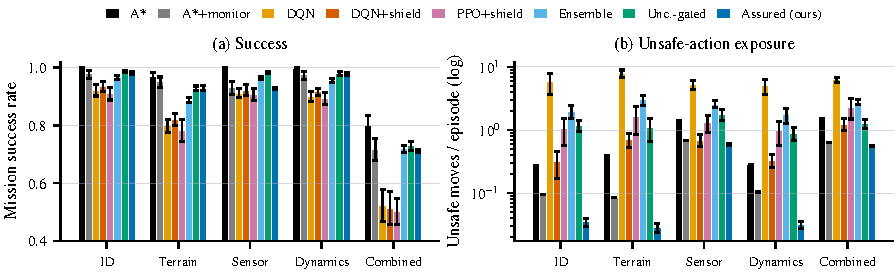
\includegraphics[width=\textwidth]{fig3_success_unsafe}
\caption{Mission success and attempted unsafe moves per episode on procedural maps. Error bars: 95\% intervals over 10
seeds (Wilson over 500 maps for A*). The method colours are reused in Figs.~\ref{fig:ops} and~\ref{fig:realshift}.}
\label{fig:main}
\end{figure*}

\begin{table}[t]
\centering
\caption{Success / unsafe moves per episode on 500 maps (mean over 10 seeds); all conditions are shown in Fig.~\ref{fig:main}.}
\label{tab:main}
\footnotesize
\setlength{\tabcolsep}{6pt}
\begin{tabular}{@{}lcc@{}}
\toprule
Method & ID & Combined shift \\ \midrule
A*                    & .998 / .270 & .800 / 1.49 \\
A*+monitor            & .980 / .096 & .718 / .632 \\
Reactive              & .798 / 2.91 & .584 / 7.55 \\
DQN                   & .921 / 5.79 & .522 / 6.29 \\
DQN+shield            & .934 / .313 & .513 / 1.24 \\
PPO                   & .876 / 16.8 & .528 / 13.9 \\
PPO+shield            & .910 / 1.05 & .502 / 2.31 \\
Ensemble              & .966 / 1.99 & .719 / 2.76 \\
Uncertainty-gated     & .986 / 1.18 & .730 / 1.27 \\
Assured               & .982 / .035 & .712 / .561 \\
Assured, no safe stop & .987 / .063 & .749 / .677 \\ \bottomrule
\end{tabular}
\end{table}

Fig.~\ref{fig:ops}c shows how often the layer intervenes. In the ID, terrain and dynamics conditions it overrides the
policy on 5--12\% of decisions, and the fallback reaches the goal in 87--97\% of the episodes in which it acts. Safe stop
trades 0.5--5.5 points of success for 0.03--0.12 fewer unsafe moves per episode (Fig.~\ref{fig:ops}d).

\begin{figure}[t]
\centering
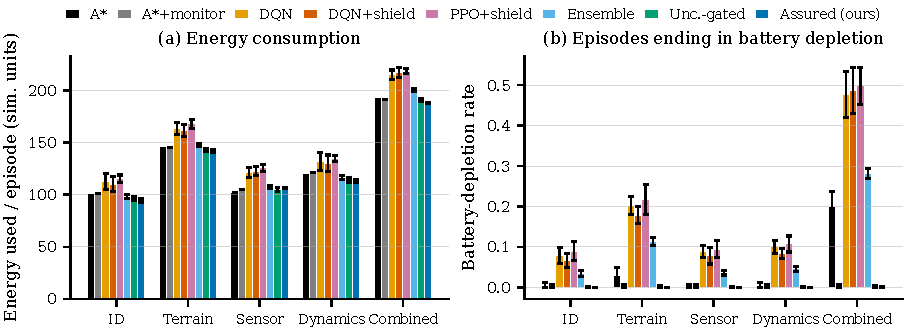
\includegraphics[width=\columnwidth]{fig4_energy}
\caption{Operational behaviour on procedural maps: energy and battery depletion for all methods (colours as in
Fig.~\ref{fig:main}), and interventions and safe stops for the assurance methods.}
\label{fig:ops}
\end{figure}

\subsection{Component Ablation}
Fig.~\ref{fig:abl} isolates the components. The safety rules provide most of the safety gain: rules alone reach 0.035
unsafe moves per episode ID, the same as the full system, and removing the rules raises unsafe moves significantly in four
of five conditions. Removing the uncertainty check lowers success by 0.9--2.7 points in the ID, terrain and dynamics
conditions, because it sends low-confidence decisions to a fallback that usually succeeds. The raw OOD check does not help:
under sensor shift it costs 3.2 points of success and adds 0.28 unsafe moves per episode (0.24 under combined shift).
Noisier readings move every observation away from the training distribution, so the check fires on 94--96\% of decisions
(Fig.~\ref{fig:ops}c), at the 90th and 99th percentile thresholds as well, and hands control to a less safe fallback.

\begin{figure}[t]
\centering
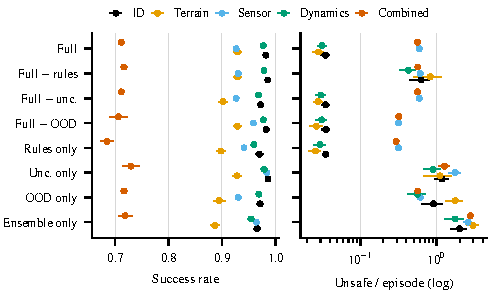
\includegraphics[width=\columnwidth]{fig6_ablation}
\caption{Ablation over all five conditions: success and attempted unsafe moves per episode (mean and 95\% CI over 10 seeds).}
\label{fig:abl}
\end{figure}

\subsection{Energy-Aware Fallback}
Replacing the fallback with an energy-blind planner (unit cell costs, constant unknown-cell premium, no feasibility check)
barely changes the pre-registered primary measure, the share of fallback episodes that avoid depletion ($+0.2$ points
under combined shift), because safe stop prevents depletion with either planner. The effect appears in
Fig.~\ref{fig:h3}: with the energy-blind fallback, success under combined shift falls from 0.71 to 0.27 because the rules
veto moves the battery can no longer afford, and energy use rises by 33--40 units under sensor and combined shift. In the
ID condition the energy-blind planner is marginally better (+1.0 point).

\begin{figure}[t]
\centering
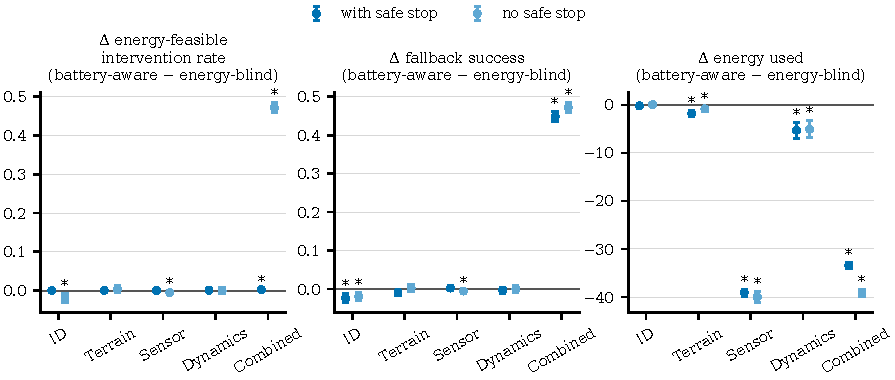
\includegraphics[width=\columnwidth]{fig8_h3}
\caption{Battery-aware minus energy-blind fallback, with and without safe stop (mean and 95\% CI over 10 seeds).}
\label{fig:h3}
\end{figure}

\subsection{Repairing the OOD Check}
\label{sec:a3}
The raw detector scores every input change, including noise the policy ignores. The action-conditioned score fires on 5.4\% of decisions under sensor shift
instead of 93.9\%, and on 20.3\% instead of 95.5\% under combined shift. Relative to the raw check (Fig.~\ref{fig:a3}),
success under sensor shift rises by 3.3 points and unsafe moves fall by 0.28 (sensor) and 0.24 (combined) per episode,
with no condition made worse. Relative to no OOD check, however, nothing changes significantly: the repair removes the
harm but does not make the OOD check useful.

\begin{figure}[t]
\centering
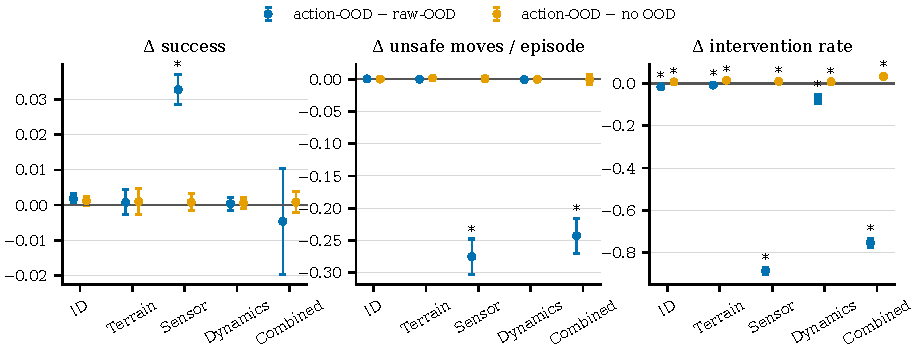
\includegraphics[width=\columnwidth]{fig9_a3}
\caption{Effect of the action-conditioned OOD score; * Holm $p<0.05$.}
\label{fig:a3}
\end{figure}

\subsection{Real-Terrain Transfer}
Fig.~\ref{fig:realshift} reports the transfer results. With nominal physics the assured system matches A* in success
(0.996 for both, not significant) with 81\% fewer unsafe moves and 3.1 fewer energy units, and beats A*+monitor on
success, unsafe moves, collisions and energy. Under shifted physics A* regains a significant success advantage of 0.4,
2.9 and 3.7 points (dynamics, sensor, combined), although the assured system still attempts 53--84\% fewer unsafe moves.
Under sensor and combined shift the raw OOD check again fires on about 90\% of decisions; the action-conditioned variant
fires on 3--4\% and lowers unsafe moves from 0.18 to 0.12 per episode. On one Gale tile under combined shift (Fig.~\ref{fig:traj}), A* follows the map edge and
collides five times when slips push it off the map, whereas the assured system hands three decisions to the fallback,
takes an interior route and reaches the goal without a collision.

\begin{figure}[t]
\centering
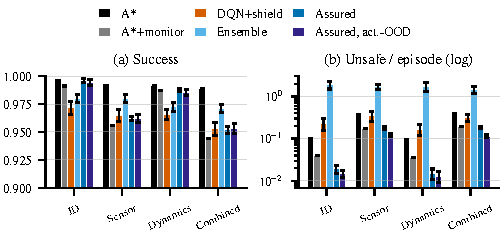
\includegraphics[width=\columnwidth]{fig11_real_shift}
\caption{Real-terrain maps under nominal and shifted physics.}
\label{fig:realshift}
\end{figure}

\begin{figure}[t]
\centering
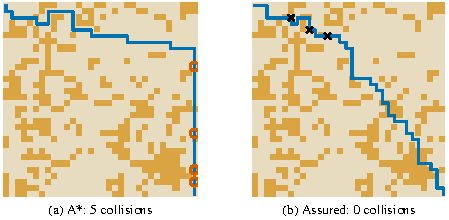
\includegraphics[width=\columnwidth]{fig12_trajectories}
\caption{Trajectories on a Gale crater tile under combined shift; circles: collisions, x: fallback.}
\label{fig:traj}
\end{figure}

% =====================================================================================================================
\section{Discussion}
The safety gain is large and consistent, but it comes almost entirely from explicit, onboard-checkable rules rather than
learned confidence, in line with the RTA preference for simple, verifiable switching conditions~\cite{hobbs2023rta}.
Rules and fallback should therefore come first, with learned-confidence checks added only where they measurably help. The
OOD results show that detecting a shift and deciding when to distrust the policy are different problems; a check that adds
value would probably need to predict failure directly. 

% =====================================================================================================================
\section{Future Work}
All findings come from a grid simulator with illustrative energy units, and the real-terrain maps take only terrain
structure from elevation data. Future work will couple the assurance layer to a physics-based rover simulator with
measured energy and slip models and evaluate it on harsher real terrain such as crater walls and dune fields. The safety
rules provide empirical rather than formal guarantees, and the uncertainty and OOD scores are uncalibrated; calibrated
failure predictors and certified safety filters are natural next steps. Finally, the follow-up experiments were designed
after the main results were known, so an independent replication on new maps and new training seeds is needed.

% =====================================================================================================================
\section{Conclusion}
This paper studied whether an onboard runtime-assurance layer can make a learned planetary-rover navigator safe to use
under partial observability and distribution shift, and which of its components matter. Under a frozen, pre-registered
protocol with 10 training seeds and 500 identical maps per condition, the layer reduced attempted unsafe moves by up to two
orders of magnitude relative to the unshielded policy, at a small cost in mission success relative to a classical
planner. Explicit, onboard safety rules provide most of this gain, while ensemble uncertainty adds a modest improvement in
success. A raw-observation OOD check is harmful under sensor shift because it reacts to noise the policy already ignores;
an action-conditioned check in the policy's own feature space removes this harm but adds no further value. An
energy-aware fallback is decisive under harsh shift, where an energy-blind fallback loses most missions. These
conclusions carry over to terrain derived from real Mars elevation data, where the assured system matches a classical
planner's success under nominal physics with far fewer unsafe moves. The results suggest that rover autonomy stacks
should build explicit rules and an energy-aware fallback first, and adopt learned confidence signals only where they are
shown to help.

\bibliographystyle{IEEEtran}
\bibliography{references}
\end{document}
